% Options for packages loaded elsewhere
\PassOptionsToPackage{unicode}{hyperref}
\PassOptionsToPackage{hyphens}{url}
\PassOptionsToPackage{dvipsnames,svgnames,x11names}{xcolor}
%
\documentclass[
  12pt]{article}

\usepackage{amsmath,amssymb}
\usepackage{iftex}
\ifPDFTeX
  \usepackage[T1]{fontenc}
  \usepackage[utf8]{inputenc}
  \usepackage{textcomp} % provide euro and other symbols
\else % if luatex or xetex
  \usepackage{unicode-math}
  \defaultfontfeatures{Scale=MatchLowercase}
  \defaultfontfeatures[\rmfamily]{Ligatures=TeX,Scale=1}
\fi
\usepackage{lmodern}
\ifPDFTeX\else  
    % xetex/luatex font selection
\fi
% Use upquote if available, for straight quotes in verbatim environments
\IfFileExists{upquote.sty}{\usepackage{upquote}}{}
\IfFileExists{microtype.sty}{% use microtype if available
  \usepackage[]{microtype}
  \UseMicrotypeSet[protrusion]{basicmath} % disable protrusion for tt fonts
}{}
\makeatletter
\@ifundefined{KOMAClassName}{% if non-KOMA class
  \IfFileExists{parskip.sty}{%
    \usepackage{parskip}
  }{% else
    \setlength{\parindent}{0pt}
    \setlength{\parskip}{6pt plus 2pt minus 1pt}}
}{% if KOMA class
  \KOMAoptions{parskip=half}}
\makeatother
\usepackage{xcolor}
\setlength{\emergencystretch}{3em} % prevent overfull lines
\setcounter{secnumdepth}{5}
% Make \paragraph and \subparagraph free-standing
\makeatletter
\ifx\paragraph\undefined\else
  \let\oldparagraph\paragraph
  \renewcommand{\paragraph}{
    \@ifstar
      \xxxParagraphStar
      \xxxParagraphNoStar
  }
  \newcommand{\xxxParagraphStar}[1]{\oldparagraph*{#1}\mbox{}}
  \newcommand{\xxxParagraphNoStar}[1]{\oldparagraph{#1}\mbox{}}
\fi
\ifx\subparagraph\undefined\else
  \let\oldsubparagraph\subparagraph
  \renewcommand{\subparagraph}{
    \@ifstar
      \xxxSubParagraphStar
      \xxxSubParagraphNoStar
  }
  \newcommand{\xxxSubParagraphStar}[1]{\oldsubparagraph*{#1}\mbox{}}
  \newcommand{\xxxSubParagraphNoStar}[1]{\oldsubparagraph{#1}\mbox{}}
\fi
\makeatother


\providecommand{\tightlist}{%
  \setlength{\itemsep}{0pt}\setlength{\parskip}{0pt}}\usepackage{longtable,booktabs,array}
\usepackage{calc} % for calculating minipage widths
% Correct order of tables after \paragraph or \subparagraph
\usepackage{etoolbox}
\makeatletter
\patchcmd\longtable{\par}{\if@noskipsec\mbox{}\fi\par}{}{}
\makeatother
% Allow footnotes in longtable head/foot
\IfFileExists{footnotehyper.sty}{\usepackage{footnotehyper}}{\usepackage{footnote}}
\makesavenoteenv{longtable}
\usepackage{graphicx}
\makeatletter
\newsavebox\pandoc@box
\newcommand*\pandocbounded[1]{% scales image to fit in text height/width
  \sbox\pandoc@box{#1}%
  \Gscale@div\@tempa{\textheight}{\dimexpr\ht\pandoc@box+\dp\pandoc@box\relax}%
  \Gscale@div\@tempb{\linewidth}{\wd\pandoc@box}%
  \ifdim\@tempb\p@<\@tempa\p@\let\@tempa\@tempb\fi% select the smaller of both
  \ifdim\@tempa\p@<\p@\scalebox{\@tempa}{\usebox\pandoc@box}%
  \else\usebox{\pandoc@box}%
  \fi%
}
% Set default figure placement to htbp
\def\fps@figure{htbp}
\makeatother

\addtolength{\oddsidemargin}{-.5in}%
\addtolength{\evensidemargin}{-1in}%
\addtolength{\textwidth}{1in}%
\addtolength{\textheight}{1.7in}%
\addtolength{\topmargin}{-1in}%
\makeatletter
\@ifpackageloaded{caption}{}{\usepackage{caption}}
\AtBeginDocument{%
\ifdefined\contentsname
  \renewcommand*\contentsname{Table of contents}
\else
  \newcommand\contentsname{Table of contents}
\fi
\ifdefined\listfigurename
  \renewcommand*\listfigurename{List of Figures}
\else
  \newcommand\listfigurename{List of Figures}
\fi
\ifdefined\listtablename
  \renewcommand*\listtablename{List of Tables}
\else
  \newcommand\listtablename{List of Tables}
\fi
\ifdefined\figurename
  \renewcommand*\figurename{Figure}
\else
  \newcommand\figurename{Figure}
\fi
\ifdefined\tablename
  \renewcommand*\tablename{Table}
\else
  \newcommand\tablename{Table}
\fi
}
\@ifpackageloaded{float}{}{\usepackage{float}}
\floatstyle{ruled}
\@ifundefined{c@chapter}{\newfloat{codelisting}{h}{lop}}{\newfloat{codelisting}{h}{lop}[chapter]}
\floatname{codelisting}{Listing}
\newcommand*\listoflistings{\listof{codelisting}{List of Listings}}
\makeatother
\makeatletter
\makeatother
\makeatletter
\@ifpackageloaded{caption}{}{\usepackage{caption}}
\@ifpackageloaded{subcaption}{}{\usepackage{subcaption}}
\makeatother

\usepackage[]{natbib}
\bibliographystyle{agsm}
\usepackage{bookmark}

\IfFileExists{xurl.sty}{\usepackage{xurl}}{} % add URL line breaks if available
\urlstyle{same} % disable monospaced font for URLs
\hypersetup{
  pdftitle={Research on Research on Research: Analyzing historical trends in statistical and computational research from the 1990s to modern day},
  pdfauthor={Naren Prakash},
  pdfkeywords={retrospective analysis, arXiv, publication analysis,
forecasting, time series},
  colorlinks=true,
  linkcolor={blue},
  filecolor={Maroon},
  citecolor={Blue},
  urlcolor={Blue},
  pdfcreator={LaTeX via pandoc}}



\begin{document}


\def\spacingset#1{\renewcommand{\baselinestretch}%
{#1}\small\normalsize} \spacingset{1}


%%%%%%%%%%%%%%%%%%%%%%%%%%%%%%%%%%%%%%%%%%%%%%%%%%%%%%%%%%%%%%%%%%%%%%%%%%%%%%

\date{March 20, 2025}
\title{\bf Research on Research on Research: Analyzing historical trends
in statistical and computational research from the 1990s to modern day}
\author{
Naren Prakash\thanks{The author gratefully acknowledges Professor Lew
for their encouragement and advice regarding the production of this
paper.}\\
Department of Statistics and Data Science, University of California, Los
Angeles\\
}
\maketitle

\bigskip
\bigskip
\begin{abstract}
This paper aims to analyze the changes in research paper output for
different statistical and computational fields over the time period from
the 1990s to modern day (2025). The paper also projects short term
growth for recently emerging fields in an effort to predict the fields
that will receive further resource funding and attention in the near
future. The research papers used for this analysis are sourced from a
dataset of papers sourced from the pre-print journal arXiv.
\end{abstract}

\noindent%
{\it Keywords:} retrospective analysis, arXiv, publication analysis,
forecasting, time series
\vfill

\newpage
\spacingset{1.9} % DON'T change the spacing!


\section{Introduction}\label{sec-intro}

In recent years, with the fields of artificial intelligence and machine
learning becoming important parts of the public lexicon and increasingly
becoming involved in our day to day lives, we have witnessed significant
changes in statistical and computational research. With statistical
methods increasingly becoming intertwined with computational principles,
such as its integration with aspects of computer science, the future of
statistics and computation appear to be one and the same. How does this
current research landscape compare with that of the landscape a mere 30
years ago? This paper aims to analyze historical trends in statistical
and computational research, as tracked by papers submitted to the online
pre-print journal arXiv, in order to visualize the dramatic changes
we've seen over the years and find any subfields growing in the present
that could yet transform the landscape of the future. This analysis of
historical trends will be conducted using a specific dataset available
on Kaggle \citet{arXiv:kaggle:data}.

\section{Literature Review}\label{lit-review}

Looking at themes in statistical and computational research is nothing
new. For instance, \citet{gelm:veht:2021} analyzed the dominant
statistical ideas of the past 50 years, suggesting inferential methods,
computational algorithms, and data analysis have been the most impactful
in the shifting of the research landscape. Smaller subsets of time have
also been analyzed, with \citet{jun:yoo:choi:2018} using Google Trends
to track the growth of different subfields of research (with an emphasis
on big data and application). This paper aims to look at a similar
problem with a different lens, using publication outputs themselves as a
way of analyzing changes in research focus and interest. In doing this,
the paper aims to also obtain an indication of the subfields with
increasing research interest in the short term that may lend itself to
future publications. Evaluating the research trends of the future has
often involved modeling itself, such as the hype cycle model
\citet{dedehayir:2016}. This model aims to track the life cycle of
technological innovations. In a similar vein, this paper aims to use
current and recent paper production output to indicate trends of the
near future. As the methodology involves using the research paper
pre-prints themselves, it may provide a clearer picture of specific
publication interests and trends rather than topics and concepts in
general.

\section{Research Questions}\label{sec-questions}

\begin{itemize}
\tightlist
\item
  What statistical and computational fields have seen the largest
  increase in publications?
\item
  How have the most published statistical and computational fields
  changed over time?
\item
  What statistical and computational fields are projected to grow the
  most in the coming years?
\end{itemize}

\section{Data}\label{sec-data}

\subsection{Data Description}\label{data-description}

The arXiv paper dataset consists of 136,238 observations and 10 columns.
The ten columns present in the data are: id, title, category, category
code, published date, updated date, authors, first author, summary, and
summary word count. Only the summary word count is a numeric variable.
This data is scraped directly from arXiv, aiming to provide a
representative sample of research published on the platform.

\subsection{Data Pre-processing}\label{data-pre-processing}

The original dataset will have its variables converted to categorical
variables for grouping and analytical purposes, with the exception of
the summary word count due to its numeric nature. Following this, two
selected lists of subtopics will be created for the purpose of data
partitioning and separate analysis.

\subsection{Data Partitioning}\label{data-partitioning}

While acknowledging the connected nature of statistical and
computational research in the present and future, this paper will
partition the data into two halves. One half will be comprised of
research deemed statistical in nature, and the other half will be
comprised of research deemed as computational. This split in the data is
done to narrow down the problem and allow for ease of analysis and
interpretation of the results. Along with this, the data will also be
subset in terms of time. In order to keep each yearly subset of papers
as a representative sample of all research output for that year, the
time range will be limited to exclude publication in 2025. This is done
so that the resulting analysis will focus on comparison with full yearly
samples of research data, rather than extrapolating from the research
output in the year 2025 as of now.

\section{Methods}\label{sec-meth}

\subsection{Quantifying growth}\label{quantifying-growth}

For the purposes of this paper, growth will be represented by two
metrics. Firstly, the simple percentage change from year to year for
each subfield will be considered. In addition to this, the proportion of
overall research represented by each subfield over time will also be
used to evaluate growth in research interest and output.

\subsection{Trend analysis and short-term
prediction}\label{trend-analysis-and-short-term-prediction}

Lastly, the metrics of growth as well as the partitioned data will be
used to create a prediction model for the short term growth of research
subfields. In correspondence with the data partitioning, separate models
will be constructed for the statistical research and the computational
research. The objective here is to produce a time series model for short
term projections of growth in research interests and outputs.

\subsection{Limitations}\label{limitations}

Focusing on primarily numerical data as a sign of growth indicates a
relatively simple way of quantifying growth. In reality, growth is a
more complex idea and could benefit from the use of paper content
through text data processing to supplement the numerical growth figures.
This is a potential avenue of further exploration and work.

\section{Results}\label{sec-results}

\subsection{Exploratory Data Analysis}\label{exploratory-data-analysis}

\subsubsection{Original Data}\label{original-data}

Before examining each partition of the original data for the purpose of
directly answering the research questions, it is important to understand
the context behind and the general appearance of the original dataset
itself. For this reason, many plots were created to visualize parts of
the data during the data pre-processing and data partitioning stages.

\begin{figure}[H]

{\centering \pandocbounded{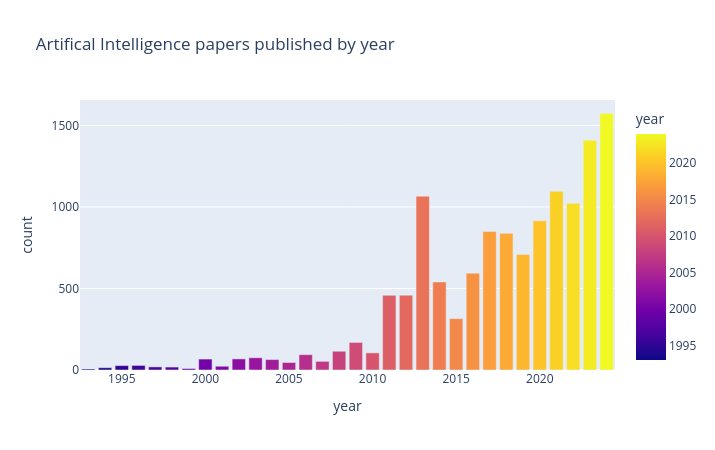
\includegraphics[keepaspectratio]{images/ai_plot-3.png}}

}

\caption{Artificial Intelligence Paper Output Plot}

\end{figure}%

This initial plot of the research paper outputs for the category of
Artificial Intelligence indicates several patterns we will continue to
see in this data. Though Artificial Intelligence is often seen as a
recent breakthrough that has only gotten larger year by year, we can see
here that the yearly trend is far from consistent.

From here, we then further explore each of the partitioned datasets
rather than focusing on the original alone, as these will be the
foundation of our future analysis and modeling.

\subsubsection{Statistical Data}\label{statistical-data}

The statistical data subset is comprised of the following topics: Data
Analysis, Statistics and Probability, Machine Learning (Statistics),
Methodology (Statistics), Computation (Statistics), Other Statistics,
Applications (Statistics), and Statistics Theory. In order to explore
the relative frequencies of paper output by these topics, we present an
initial plot of this data.

\begin{figure}[H]

{\centering \pandocbounded{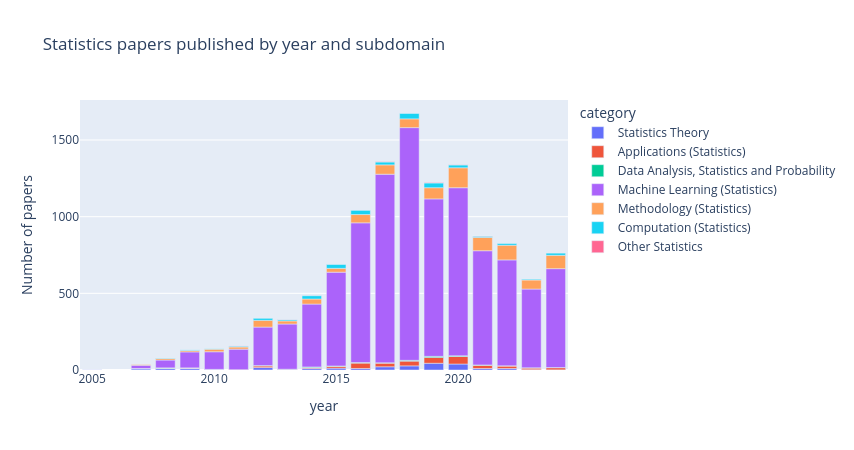
\includegraphics[keepaspectratio]{images/stat_edaplot-2.png}}

}

\caption{Statistical Data Paper Output Plot}

\end{figure}%

From this initial plot it is immediately apparent that Machine Learning
(Statistics) and Methodology appear to be the most popular subdomains,
with other subdomains varying and not having a clear edge over each
other. This provides us with a general impression of the data prior to
delving into the specific yearly figures and relative frequencies.

\subsubsection{Computational Data}\label{computational-data}

The computational data subset is made up from the following topics:
Artificial Intelligence; Computation and Language (Legacy category);
Computation and Language (Natural Language Processing); Computer Vision
and Pattern Recognition; Distributed, Parallel, and Cluster Computing;
Neural and Evolutionary Computing; Computer Science and Game Theory; and
Computational Physics. Once more, we create an initial plot to explore
the relative frequencies of paper output by subfield.

\begin{figure}[H]

{\centering \pandocbounded{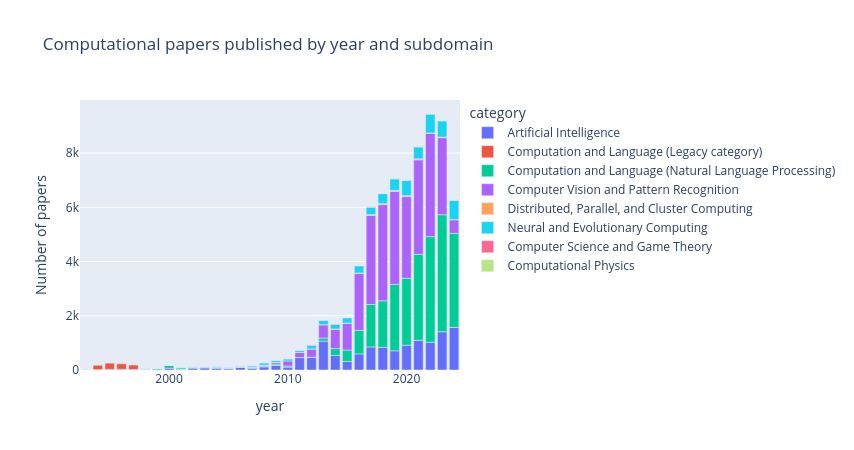
\includegraphics[keepaspectratio]{images/comp_edaplot.png}}

}

\caption{Computational Data Paper Output Plot}

\end{figure}%

Once more, we can see a few subtopics are the most popular visually. In
this case, the Computer Vision and Pattern Recognition, Computation and
Language (Natural Language Processing), and the Artificial Intelligence
subtopics have the highest proportions of paper outputs, especially in
more recent years. This is not unexpected, considering the rise of LLMs
and the popularity of Artificial Intelligence in modern society.

\subsection{Statistical Data Analysis}\label{statistical-data-analysis}

\subsubsection{Fields with the largest publication
increase}\label{fields-with-the-largest-publication-increase}

In order to quantify the largest publication increase for the
statistical fields, two methods were employed. One method involved
looking at the average growth (in percentages) year over year for each
subtopic. The other involved comparing the raw paper output from the
first year of comparison for each subtopic to its more recent paper
output total. The results of both forms of analysis are shown in the
following plots.

\begin{figure}[H]

{\centering \pandocbounded{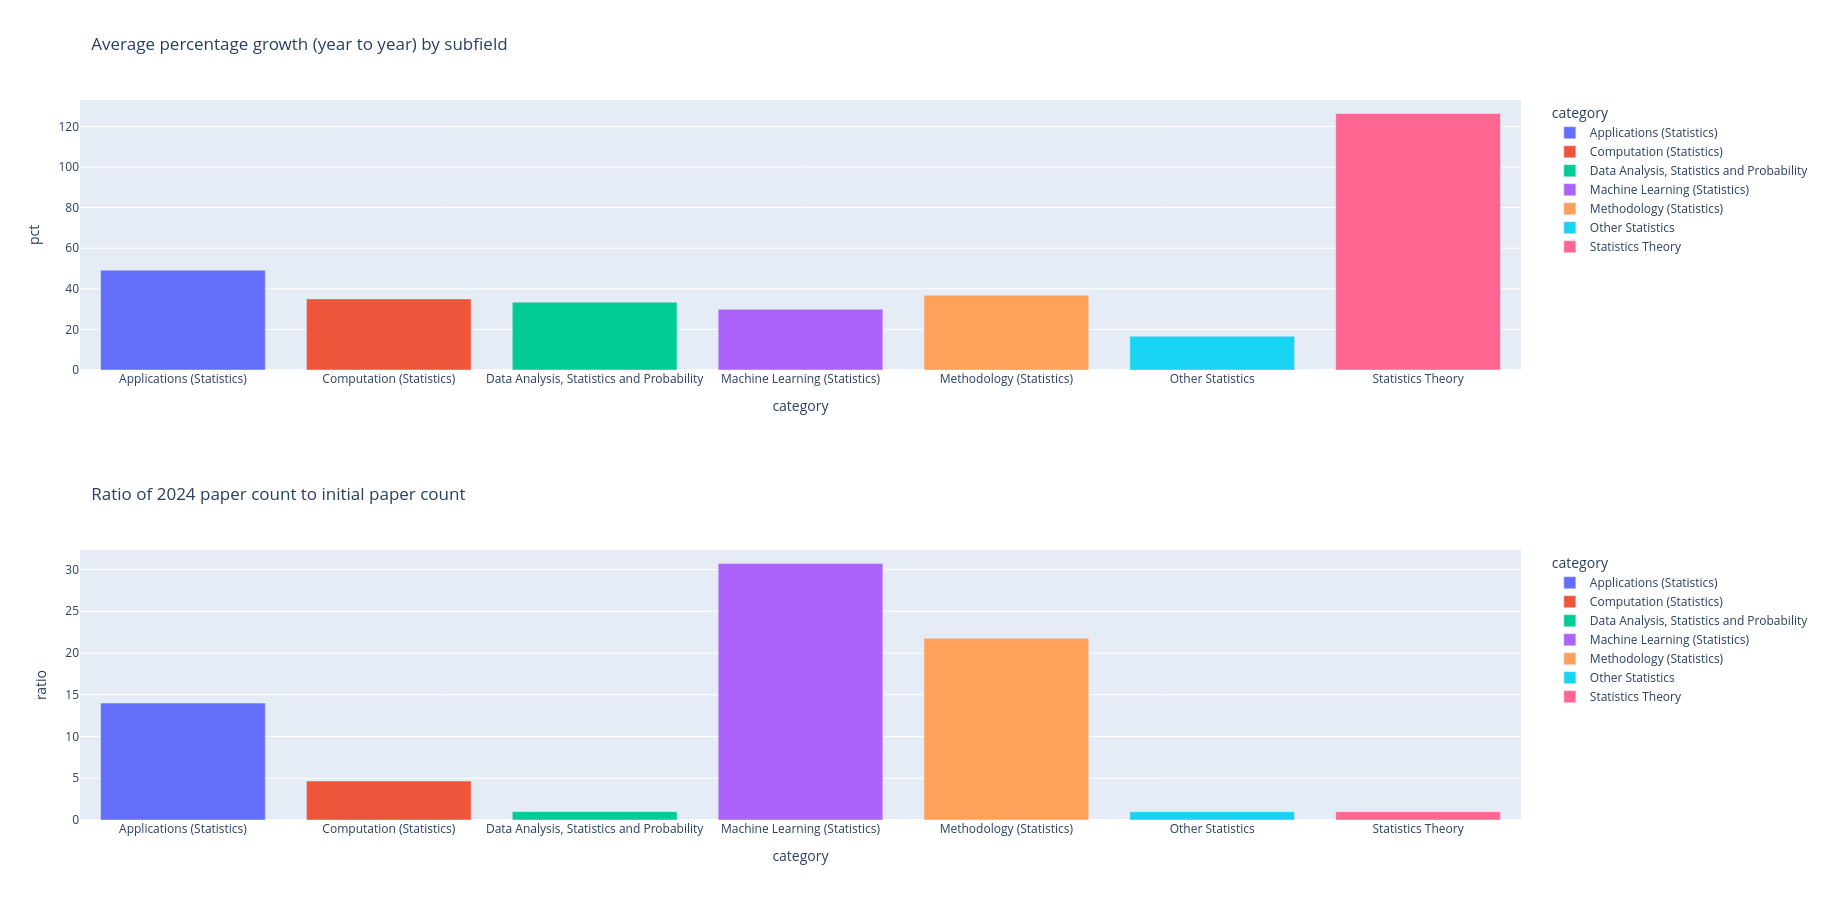
\includegraphics[keepaspectratio]{images/ratio_stats-imageonline.co-merged(1).png}}

}

\caption{Statistical Data Average Growth and Ratio Plots}

\end{figure}%

Based on the two plots above, we can see some patterns as many of the
subfields retain the same order in both the paper output ratio and the
average yearly percentage growth. The apparent exception here is
Statistics Theory, which despite having an extremely high percentage
growth year by year, is among the lowest for growth in terms of raw
totals. The reason for this, after further investigation, is due to the
volatile nature of Statistics Theory publications on a yearly basis, as
many years would have little published but be followed by a year with a
larger output. This inconsistency produced a very large average
percentage growth yet an overall small increase in raw output. From
considering these graphs, we can see that the fields with the most
growth in this time period are Machine Learning, Methodology, and
Applications.

\subsubsection{Changes in the top fields over the
years}\label{changes-in-the-top-fields-over-the-years}

In order to analyze publication output on a yearly basis, the top 4
subfields in paper output for a given year were calculated and plotted.
The visualization produced from this is below.

\begin{figure}[H]

{\centering \pandocbounded{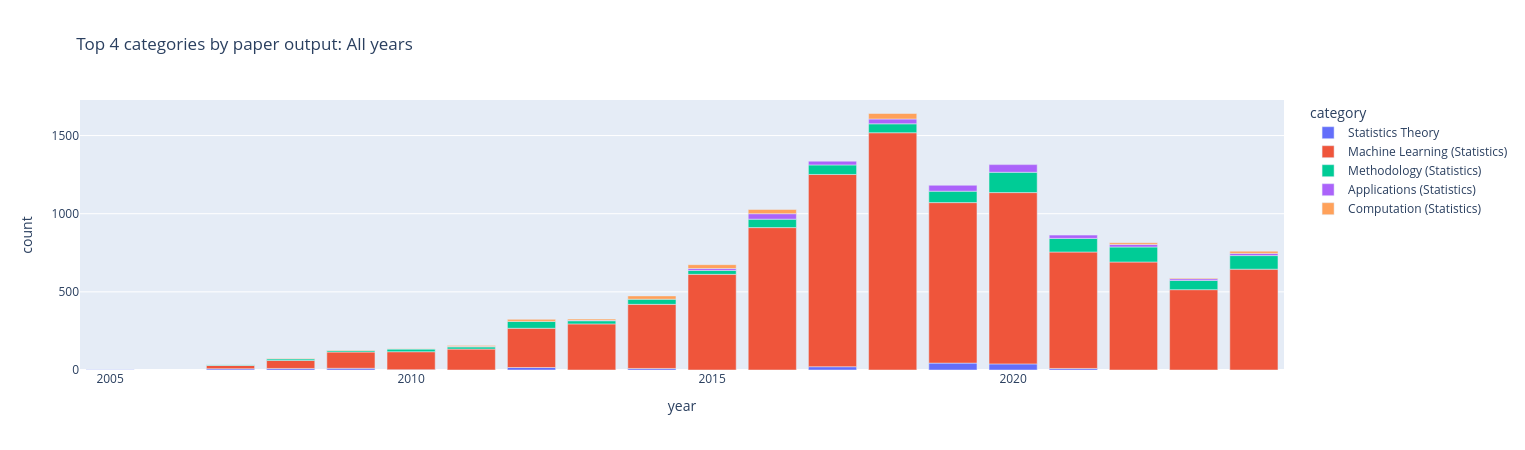
\includegraphics[keepaspectratio]{images/top4_stats.png}}

}

\caption{Statistical Data Top 4 Subfields Yearly}

\end{figure}%

From this analysis, we can see that the most published subfields
remained consistent over the years. Machine Learning, Methodology,
Applications, and Computation often comprised the top 4 with Statistics
Theory also in the mix. Overall, the top 3 fields remained Machine
Learning, Methodology, and Application / Computation with some variance
between the presence of Application and Computation in any individual
year.

\subsubsection{Projected growth of statistical
fields}\label{projected-growth-of-statistical-fields}

In order to tackle the short term prediction of paper outputs, we will
examine recent trends in publications. An initial look at this is
through limiting the time frame. Here we restrict the data from
2015-2024 and look at the average percentage growth in publication
output.

\begin{figure}[H]

{\centering \pandocbounded{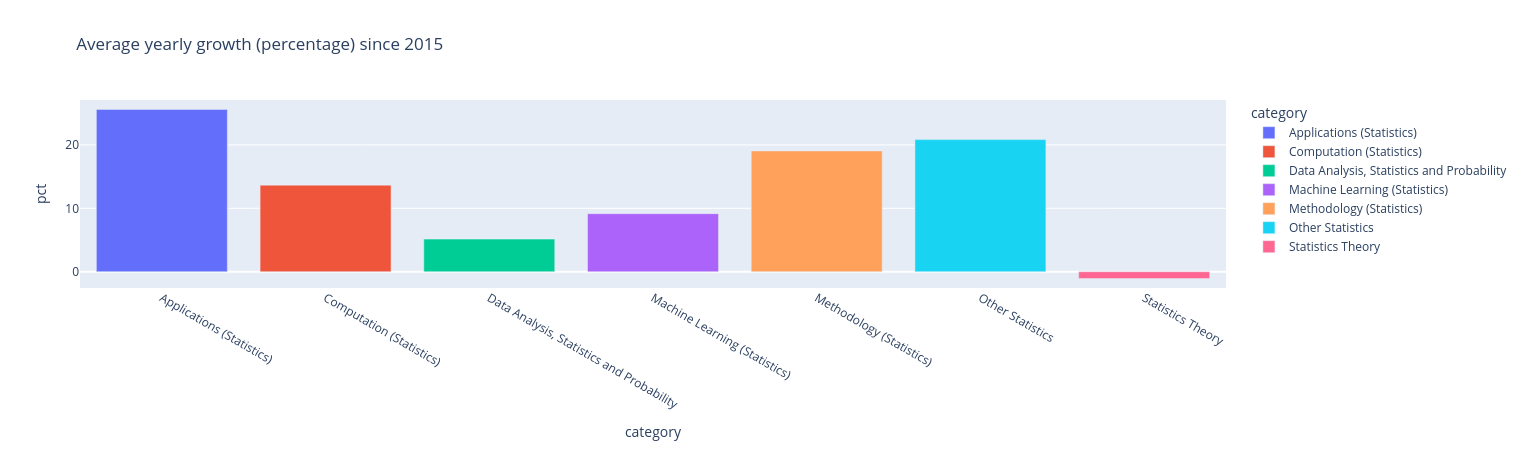
\includegraphics[keepaspectratio]{images/stats_recent.png}}

}

\caption{Statistical Data Recent Publication Growth}

\end{figure}%

From this, we can see that publication growth is actually highest in
Other Statistics, Methodology, and Applications. Somewhat surprisingly,
the publication average growth of the Machine Learning subfield is
relatively low. In order to fully capture the historical trends and use
them for future predictions, we want to utilize a time series approach.

\subsubsection{Creating the time series
model}\label{creating-the-time-series-model}

In order to create a suitable model for the future time series
prediction of paper outputs by subfield, we first need to understand the
relationships between subfields. We first look at the correlation
between each subfield to understand if the patterns in paper output are
dependent on other subfields.

\begin{figure}[H]

{\centering \pandocbounded{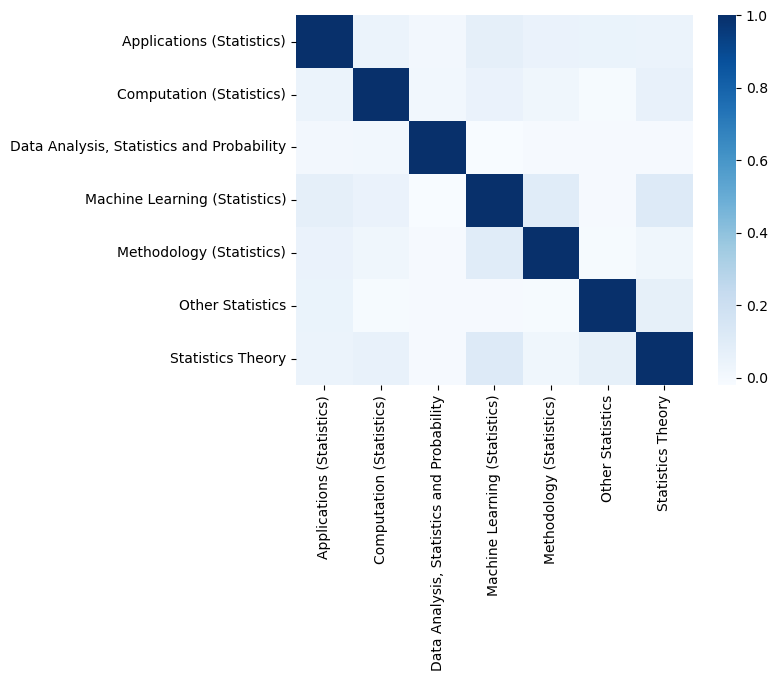
\includegraphics[keepaspectratio]{images/stats_corr.png}}

}

\caption{Statistical Data Correlation Heatmap}

\end{figure}%

From this heatmap, we can conclude that each subfield is largely
independent of other subfields, with the correlation values across
subfields being fairly low. As a result, we choose a model that predicts
future values based on the previous values of each individual subfield.
Essentially, we treat each subfield as an individual time series.

The model itself is constructed using the skforecast package from
\citet{skforecast}. We use a LightGBM regressor to create a
ForecasterAutoregMultiSeries object from the aforementioned skforecast
library. From previous fitting of a Vector Autoregression Model, we
specify 9 lag periods for the object.

We create a training set from the statistical data of the first 70\% of
observations, with the remaining 30\% serving as the test set. After
training and predicting on our test set, we see a mean absolute error of
about 0.5913. Finally, we use all the original data as the training data
for a model object identical to that of our original and supply the
future time frame of the first 6 months of 2025. From those predictions,
the following trends are seen.

\begin{figure}[H]

{\centering \pandocbounded{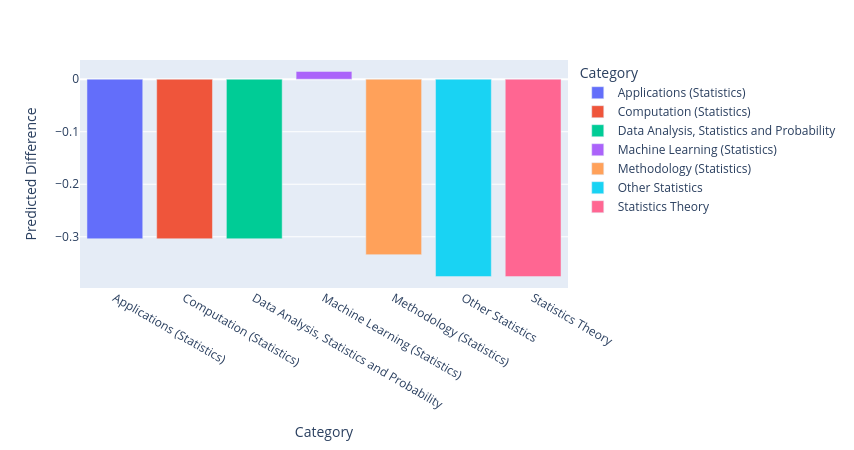
\includegraphics[keepaspectratio]{images/stat_preds.png}}

}

\caption{Statistical Data Predicted Differences}

\end{figure}%

As seen here, the time series model predicts a decline in paper output
for each subfield over the first 6 months of 2025, with the exception
being in Machine Learning. Further inspection into the changes of the
percentages over time show an inconsistent rate of change, with many ups
and downs.

This further analysis shows a trend commonly seen in the predictions of
each of the individual subfields. Considering the nature of the
statistical data from our observations, it seems apt that the
predictions themselves also reflect the inconsistency seen in paper
output. Ultimately, from these predictions, in the short term Machine
Learning is expected to see the most paper output.

\subsection{Computational Data
Analysis}\label{computational-data-analysis}

\subsubsection{Fields with the largest publication
increase}\label{fields-with-the-largest-publication-increase-1}

Once more, we use the same two methods to quantify this. We look at
average growth (in percentages) year over year for each subtopic before
then comparing the raw paper output from the first year of comparison
for each subtopic to its more recent paper output total. The two plots
below show us the results.

\begin{figure}[H]

{\centering \pandocbounded{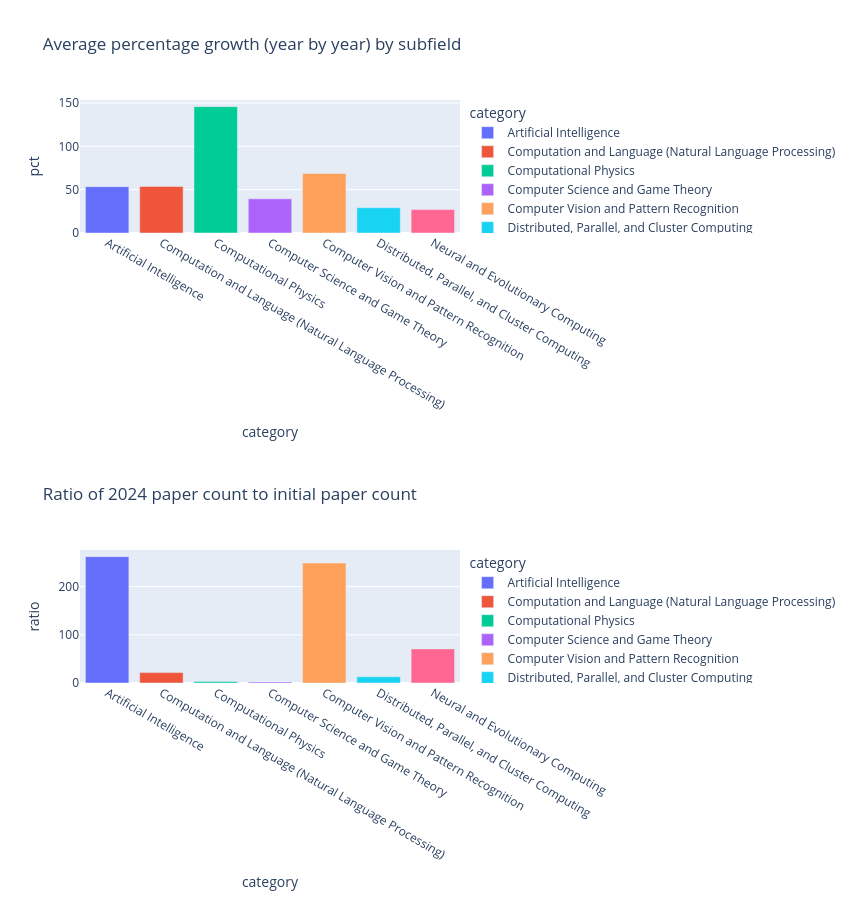
\includegraphics[keepaspectratio]{images/ratio_comp-imageonline.co-merged.png}}

}

\caption{Computational Data Average Growth and Ratio Plots}

\end{figure}%

Similar to Statistics Theory in our statistical data yearly growth plot,
Computational Physics has the highest average growth but a small ratio,
indicating that it is the most volatile subfield with publication
outputs varying between relatively small and relatively large. These
plots indicate that Artificial Intelligence, Computer Vision, and Neural
and Evolutionary Computing are the largest subfields.

\subsubsection{Changes in the top fields over the
years}\label{changes-in-the-top-fields-over-the-years-1}

\begin{figure}[H]

{\centering \pandocbounded{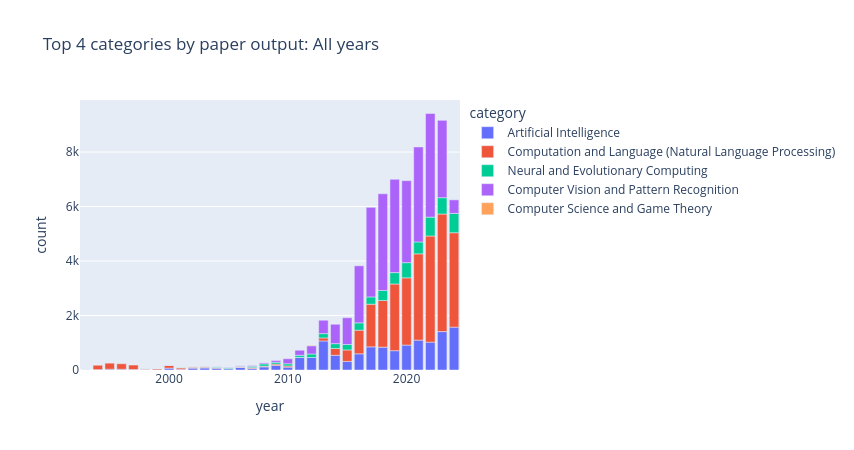
\includegraphics[keepaspectratio]{images/top4_comp.png}}

}

\caption{Computational Data Top 4 Subfields Yearly}

\end{figure}%

From this, we can see that the subfields comprising the majority of
computational papers have been Artificial Intelligence, Computation and
Language (Natural Language Processing), and Computer Vision and Pattern
Recognition. Perhaps surprisingly, the Artificial Intelligence subfield
has been one of the larger subfields for much longer than its stay in
the public lexicon. Despite it only recently becoming known to the
general public, the research output indicates it has been an emerging
and popular publication subfield for quite a while.

\subsubsection{Projected growth of computational
fields}\label{projected-growth-of-computational-fields}

Using a subset from 2015 to the present, the average growth of each
subfield is extremely similar to that displayed in Figure 9. Thus, to
gain additional insight into the projected growth of the computational
fields in question, we turn toward the time series model once again.

\subsubsection{Creating the time series
model}\label{creating-the-time-series-model-1}

We again choose a model that predicts future values based on the
previous values of each individual subfield due to a weak correlation
between the subfields.

The model itself is constructed using the skforecast package from
\citet{skforecast}. We use a LightGBM regressor to create a
ForecasterAutoregMultiSeries object from the aforementioned skforecast
library. From previous fitting of a Vector Autoregression Model, we
specify 13 lag periods for this object.

We create a training set from the statistical data of the first 70\% of
observations, with the remaining 30\% serving as the test set. After
training and predicting on our test set, we see a mean absolute error of
about 2.0295. Notably, we can see that our model is less accurate in
predicting the differences in computational fields as compared to the
similar model used for the statistical data. We then use all the
original data as the training data for a model object identical to that
of our original and supply the future time frame of the first 6 months
of 2025. The predicted trends are seen below.

\begin{figure}[H]

{\centering \pandocbounded{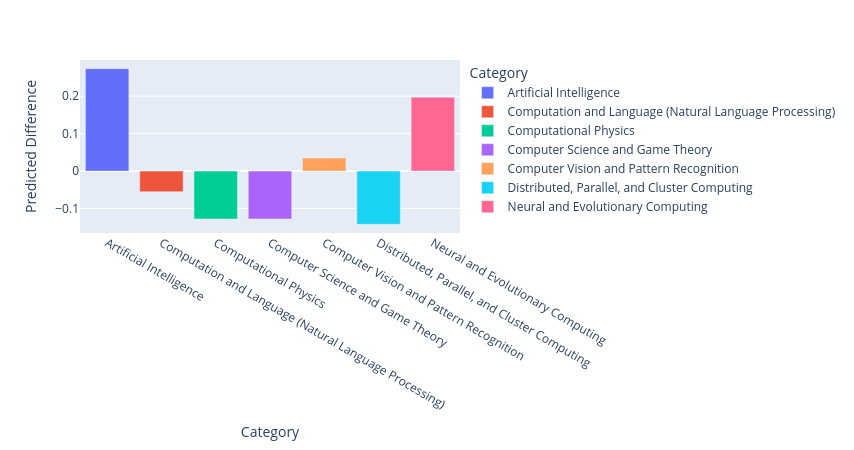
\includegraphics[keepaspectratio]{images/comp_preds.png}}

}

\caption{Computational Data Predicted Differences}

\end{figure}%

From our time series model, we see a projected growth in publication
output for Artificial Intelligence, Neural and Evolutionary Computing,
and a smaller growth for Computer Vision and Pattern Recognition. This
model projects more publication growth than the comparable statistical
data model, which only projected growth for one subfield. However, it is
important to note that the mean absolute error for this model is larger,
and as such the model predictions may be less accurate.

\section{Conclusion}\label{sec-conc}

From looking at the various statistical and computational subfields from
the 1990s to the present day, we can see that the popularity of research
and paper output for subfields remains fairly consistent. While the
actual outputs, as in the raw paper totals, vary a lot year by year, the
top subfields tend to keep their places. For statistical data that was
Machine Learning, Methodology, Applications, and Computation. For
computational data, that was Computation and Language (Natural Language
Processing), Artificial Intelligence, and Computer Vision and Pattern
Recognition. With that being said, there are several subfields our
models predicted to grow in the near future. The computational time
series model projected a growth in the Neural and Evolutionary Computing
subfield, a subfield not often in the top subfields in terms of paper
output. It also projected continued growth for the field of Artificial
Intelligence and to a lesser extent Computer Vision and Pattern
Recognition. On the other hand, the statistical time series model
projected continued growth for the Machine Learning subfield, while
projecting short term decreases in the output of other subfields. It is
important to note that the differences in predicted growth between the
statistical and computational models may be affected by the source of
publications used in this analysis, as arXiv hosts more computational
papers than statistical papers. As a result, future analysis may want to
incorporate several different sources and/or using oversampling
techniques to ensure comparable analysis for each subtopic.

\subsection{Potential Impact}\label{potential-impact}

The projections derived from this research can be used by both
researchers and research institutions to manage funding and promote the
growth of emerging fields of research. In addition to influencing the
innovative research of the future, the projections and analysis within
this project represent a reference point for the past and current
developments in statistical and computational research. With arXiv
becoming more popular as a pre-print journal for research in these
fields and the dynamic nature of research continuing to be
unpredictable, this paper can provide a snapshot of the research
landscape for future retrospective analysis.

\section{Source Code and Data}\label{source-code-and-data}

All code used in the production of this analysis, as well as the
original dataset from arXiv, can be found at
\href{https://github.com/narenp12/stats140finalproj}{this repository}.


  \bibliography{bibliography.bib}



\end{document}
